\documentclass[border=10pt]{standalone}
\usepackage{tikz}
\usetikzlibrary{shapes.geometric, calc}

\begin{document}
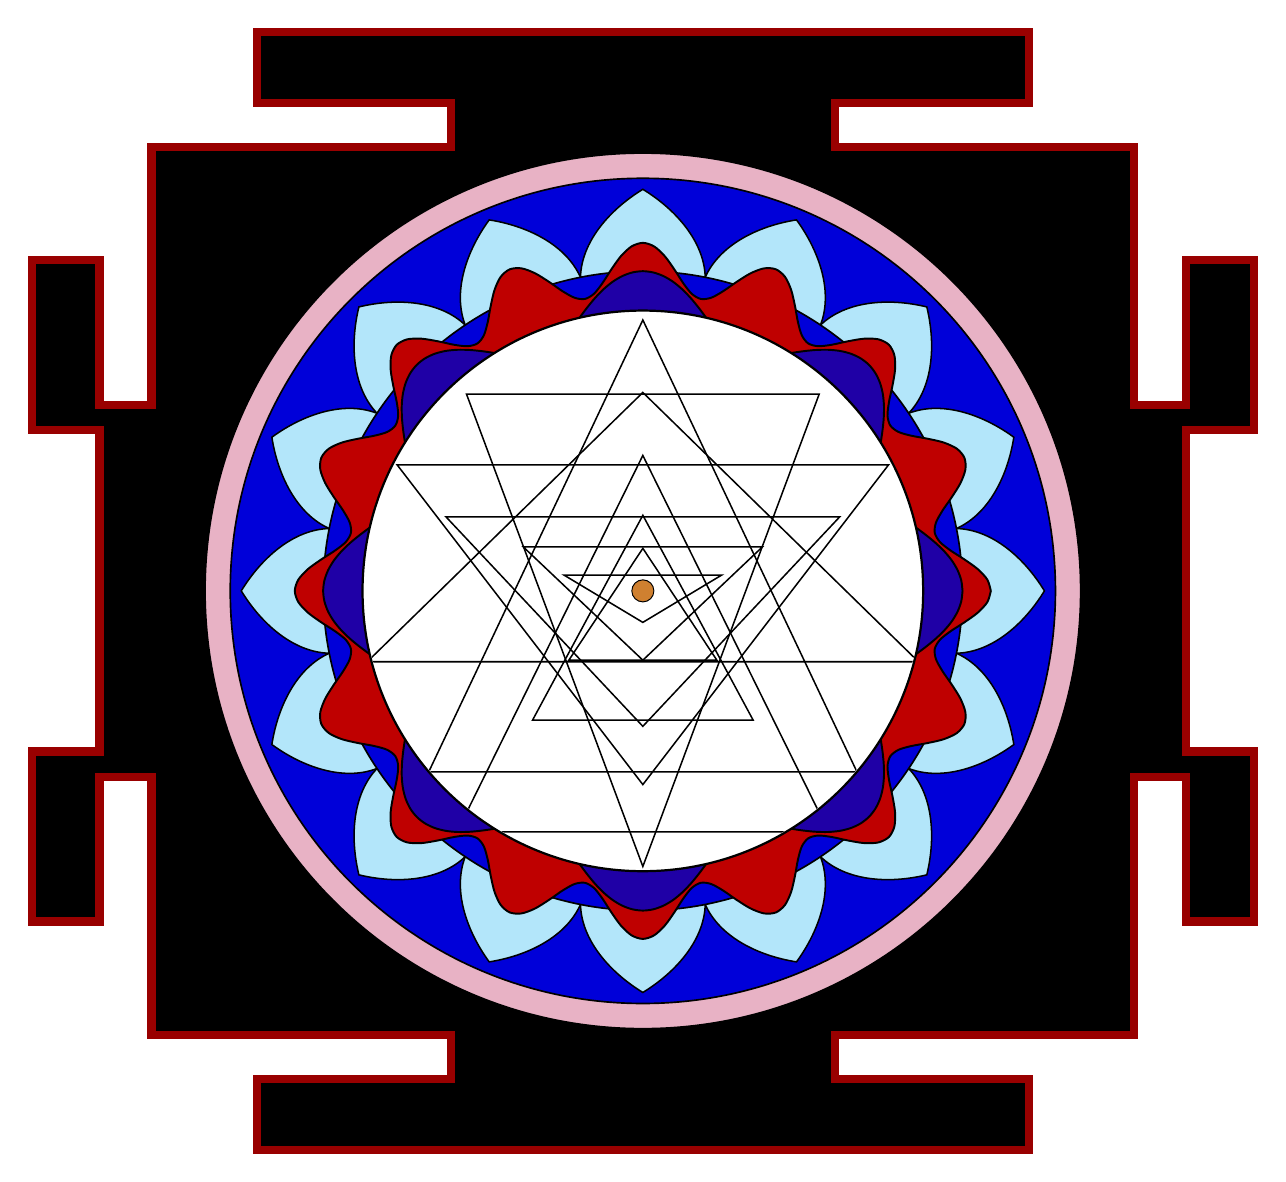
\begin{tikzpicture}[scale=2]

% Outer stepped Bhupura enclosure - black with dark red outline
\filldraw[fill=black, draw=red!60!black, line width=3pt, line join=miter]
    (-2.45,3.55) -- (2.45,3.55) -- (2.45,3.10) -- (1.22,3.10) -- (1.22,2.82) --
    (3.12,2.82) -- (3.12,1.18) -- (3.45,1.18) -- (3.45,2.10) -- (3.88,2.10) --
    (3.88,1.02) -- (3.45,1.02) -- (3.45,-1.02) -- (3.88,-1.02) -- (3.88,-2.10) --
    (3.45,-2.10) -- (3.45,-1.18) -- (3.12,-1.18) -- (3.12,-2.82) -- (1.22,-2.82) --
    (1.22,-3.10) -- (2.45,-3.10) -- (2.45,-3.55) -- (-2.45,-3.55) -- (-2.45,-3.10) --
    (-1.22,-3.10) -- (-1.22,-2.82) -- (-3.12,-2.82) -- (-3.12,-1.18) -- (-3.45,-1.18) --
    (-3.45,-2.10) -- (-3.88,-2.10) -- (-3.88,-1.02) -- (-3.45,-1.02) -- (-3.45,1.02) --
    (-3.88,1.02) -- (-3.88,2.10) -- (-3.45,2.10) -- (-3.45,1.18) -- (-3.12,1.18) --
    (-3.12,2.82) -- (-1.22,2.82) -- (-1.22,3.10) -- (-2.45,3.10) -- cycle;

% Outer lavender circle
\filldraw[fill=black!20!blue!30!red!30, draw=black, line width=0.6pt] (0,0) circle (2.78);

% Blue ring
\filldraw[fill=blue!85!black, draw=black, line width=0.6pt] (0,0) circle (2.62);

% Light blue lotus petals (16 broad pointed petals)
\foreach \angle in {0,22.5,...,337.5} {
    \filldraw[fill=cyan!30!white, draw=black, line width=0.55pt]
        ({\angle-11.25}:2.03)
        .. controls ({\angle-10}:2.25) and ({\angle-5}:2.43) .. ({\angle}:2.55)
        .. controls ({\angle+5}:2.43) and ({\angle+10}:2.25) .. ({\angle+11.25}:2.03)
        .. controls ({\angle+5}:1.88) and ({\angle-5}:1.88) .. ({\angle-11.25}:2.03);
}

% Blue circle inside petals
\filldraw[fill=blue!85!black, draw=black, line width=0.6pt] (0,0) circle (2.03);

% Red/crimson scalloped band
\filldraw[fill=red!75!black, draw=black, line width=0.7pt]
    plot[domain=0:360, samples=193, smooth cycle]
        ({(2.05 + 0.16*cos(16*\x))*cos(\x)}, {(2.05 + 0.16*cos(16*\x))*sin(\x)});

% Dark purple 8-lobed wavy ring
\filldraw[fill=black!65!red!35!blue, draw=black, line width=0.7pt]
    plot[domain=0:360, samples=193, smooth cycle]
        ({(1.83 + 0.20*cos(8*\x))*cos(\x)}, {(1.83 + 0.20*cos(8*\x))*sin(\x)});

% White central circle for Sri Yantra
\filldraw[fill=white, draw=black, line width=0.8pt] (0,0) circle (1.78);

% Sri Yantra - dense interlocking triangle construction
\begin{scope}
\clip (0,0) circle (1.77);
\draw[black, line width=0.55pt] (0,1.72) -- (-1.36,-1.15) -- (1.36,-1.15) -- cycle;
\draw[black, line width=0.55pt] (0,1.26) -- (-1.75,-0.45) -- (1.75,-0.45) -- cycle;
\draw[black, line width=0.55pt] (0,0.86) -- (-1.18,-1.53) -- (1.18,-1.53) -- cycle;
\draw[black, line width=0.55pt] (0,0.48) -- (-0.70,-0.82) -- (0.70,-0.82) -- cycle;
\draw[black, line width=0.55pt] (0,0.27) -- (-0.47,-0.44) -- (0.47,-0.44) -- cycle;

\draw[black, line width=0.55pt] (0,-1.75) -- (-1.12,1.25) -- (1.12,1.25) -- cycle;
\draw[black, line width=0.55pt] (0,-1.23) -- (-1.56,0.80) -- (1.56,0.80) -- cycle;
\draw[black, line width=0.55pt] (0,-0.86) -- (-1.25,0.47) -- (1.25,0.47) -- cycle;
\draw[black, line width=0.55pt] (0,-0.44) -- (-0.76,0.28) -- (0.76,0.28) -- cycle;
\draw[black, line width=0.55pt] (0,-0.20) -- (-0.50,0.10) -- (0.50,0.10) -- cycle;
\end{scope}

% Central bindu (brown dot)
\filldraw[fill=brown!75!orange, draw=black, line width=0.35pt] (0,0) circle (0.07);

\end{tikzpicture}
\end{document}
